\chapter{The Level-1 Trigger Online Software}
% read the paper about the cell structure
% - cell tree structure
% - web interfaces
% - panels \& SDK
% - Phase II plans

\section{The Level-1 Trigger}

The online software is designed to setup, configure, and monitor the electronics
responsible for analyzing and filtering data from the CMS experiment
as the LHC provides it with sets of proton-proton collisions in the center of
the detector at a rate of 40MHz.

The current luminosity of the beam in LHC gives an average of \~40-50
proton-proton collisions per bunch crossing, resulting in around 2MB\cite{CMS_Experiment2} of data
generated by the sensor electronics.

At a rate of 40MHz this will effectively produce a data stream of 80TB/s.
This is too much for any storage system to handle, so a system is needed to
filter this data so that only interesting events are retained.

To make the data rate manageable a set of (very fast) algorithms are executed on
hardware just outside the detector as events occur to filter out `uninteresting` data,
i.e. physics events that are already known and well-defined. This because
collision experiments have been performed for many years now and many observable
physics processes in them have already been thoroughly studied.

This filter is called the Level-1 (L1) trigger and will reduce the `event rate`
(i.e. bunch crossing containing proton-proton collisions) from 40MHz to a
relative rate of \~100kHz.

The output data stream of the L1 trigger is then forwarded to the high-level trigger
(HLT), which will reduce the event
rate from 100kHz to 100Hz. The output data from the HLT is then stored for
further analysis by the Worldwide LHC Computing Grid (WLCG).
More information about the HLT can be found in the Phase II technical proposal
\cite{TS_Phase2}.

The calculations of the L1 trigger are performed on FPGA (field-programmable
gate array) hardware.
These hardware boards follow a common firmware pipeline.
The L1 trigger is designed to make a decision every \SI{4}{\micro\second}, the
time it takes for 160 bunch crossings to occur.
The trigger will issue a Level-1 Accept (L1A) if this set of bunch crossings
is deemed interesting.

The trigger is composed of four levels.

The lowest level, called the Local Triggers or Trigger Primitive Generators (TPG),
is a set of hardware boards deployed in the calorimeters as well as the
muon chambers, where they are designed to analyze the energy readings and
recognize patterns.
This level contains the Electromagnetic Calorimeter (ECAL), the
Hadron Calorimeter (HCAL), the Cathode Strip Chambers (CSC), the
Resistive Plate Chambers (RPC), and the Drift Tube (DT).

The second level combines the information of the
Local Triggers and try to make basic reconstructions to determine what sort of
physics event has happened in that particular region of the experiment.
It outputs `trigger objects`, which signify the particle type (e.g. a passing electron or
muon) and a rank. The rank is determined by the energy, momentum, and a level of
confidence of this measurement.
This level contains the TwinMux, the Calorimeter Trigger Layer 1, the
Endcap Muon Track Finder (EMTF), the Overlap Muon Track Finder (OMTF), and the
Barrel Muon Track Finder (BMTF).

The third level, called the Global Calorimeter and Global Muon Triggers, filter
out the highest ranked trigger objects reported by the Regional Triggers.

The highest level, called the Global Trigger, determines whether or not to issue
a Level-1 Accept (L1A), and instructs the Timing Trigger and Control System (TTC)
to read out the full-precision data stored in the buffers of the FPGA hardware
inside the detector.
This level contains the Calorimeter Trigger Layer 2, the Global Muon Trigger ($\mu$GMT),
and the Global Trigger ($\mu$GT).

This trigger loop is explained visually in figure \ref{fig:l1triggerloop}.

\begin{figure}
  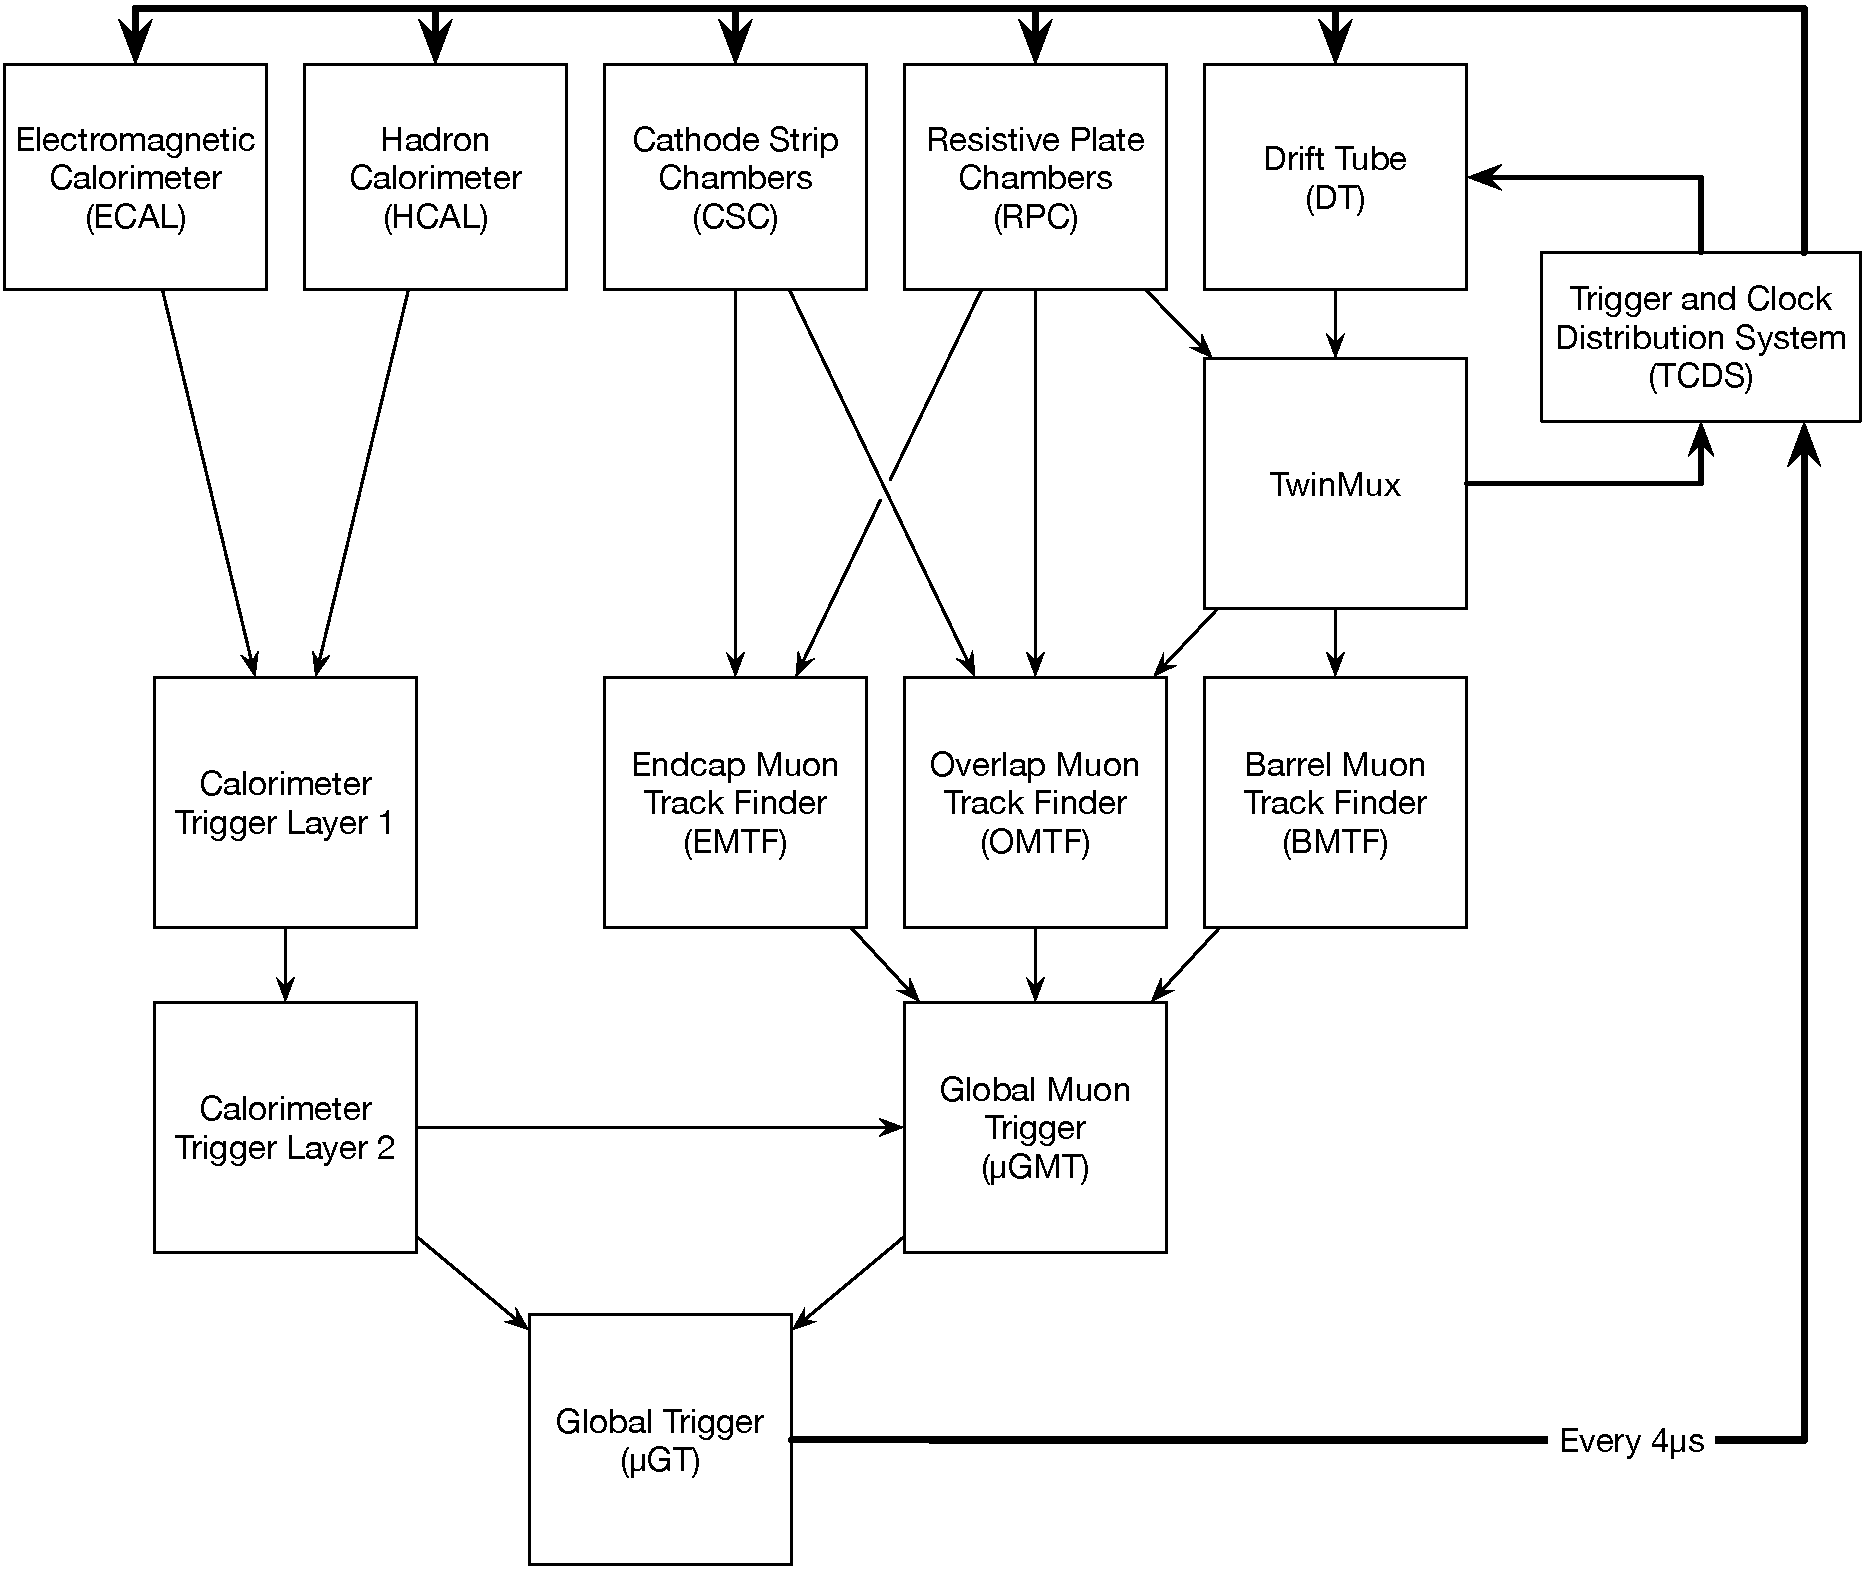
\includegraphics[width=\textwidth]{images/L1-trigger-loop}
  \caption{Conceptual drawing of the L1 trigger hardware loop}
  \label{fig:l1triggerloop}
\end{figure}

Note that, because of the decision deadline of \SI{4}{\micro\second}, the
buffers will contain data of 160 bunch crossings.

Also note that this trigger loop only considers data from calorimeters and
muon chambers to limit the data flow through the pipeline.

The Trigger and Clock Distribution System (TCDS) is in charge of distributing a L1A
and control signals (e.g. calibration, clock synchronization, test, reset, \ldots).

\section{The CMS Experiment Control System}
The CMS Experiment Control System (ECS) is a distributed software system that
is designed to manage the configuration, testing, and monitoring of all hardware
involved in the L1 trigger and DAQ system of the CMS experiment.

One of the components of ECS is the Cross Data Acquisition System, called XDAQ.
It is a custom-made data acquisition system specialized for high energy physics.
It is developed internally by the CMS group.

% It's task is to receive fragmented data about a collision event and reconstruct
% it to restore the full event.

XDAQ provides a standardized way to perform high energy physics analyses. It
provides developers with a uniform DAQ system. It hides the complexity of data
exchange and distributed computing for the developer.
It allows subsystems to load its own software modules to perform various tasks.
XDAQ also provides an interface engine each subsystem can use to render a web
interface.

\section{The Trigger Supervisor}
The Trigger Supervisor is a framework built upon XDAQ which specializes in
controlling the various aspects of the L1 trigger and providing libraries for
the execution of common tasks performed in most of the subsystems (e.g. configure, test, \ldots).
For example it provides standardized APIs for executing configuration commands and
generating monitoring data.

This composes a central system through which the status of all the subsystems
of the experiment can be monitored.

The Trigger Supervisor is, as it is built on top of XDAQ, distributed.
It is implemented in the form of a tree of `cells`.
The Trigger Supervisor has a root cell, called the Central Cell, which has
several subcells, each corresponding to a L1-trigger subsystem.
Each subcell can contain further subcells. A cell can be a hardware component,
or a controller. In the cell tree, all end nodes of the tree are hardware components.

Each cell creates its own web interface dealing with that cell's particular
functionality. This way a user can use the web interface to receive a general
overview of a system, and traverse the tree to get more specific data and
functionality.

\begin{figure}
  \centering
  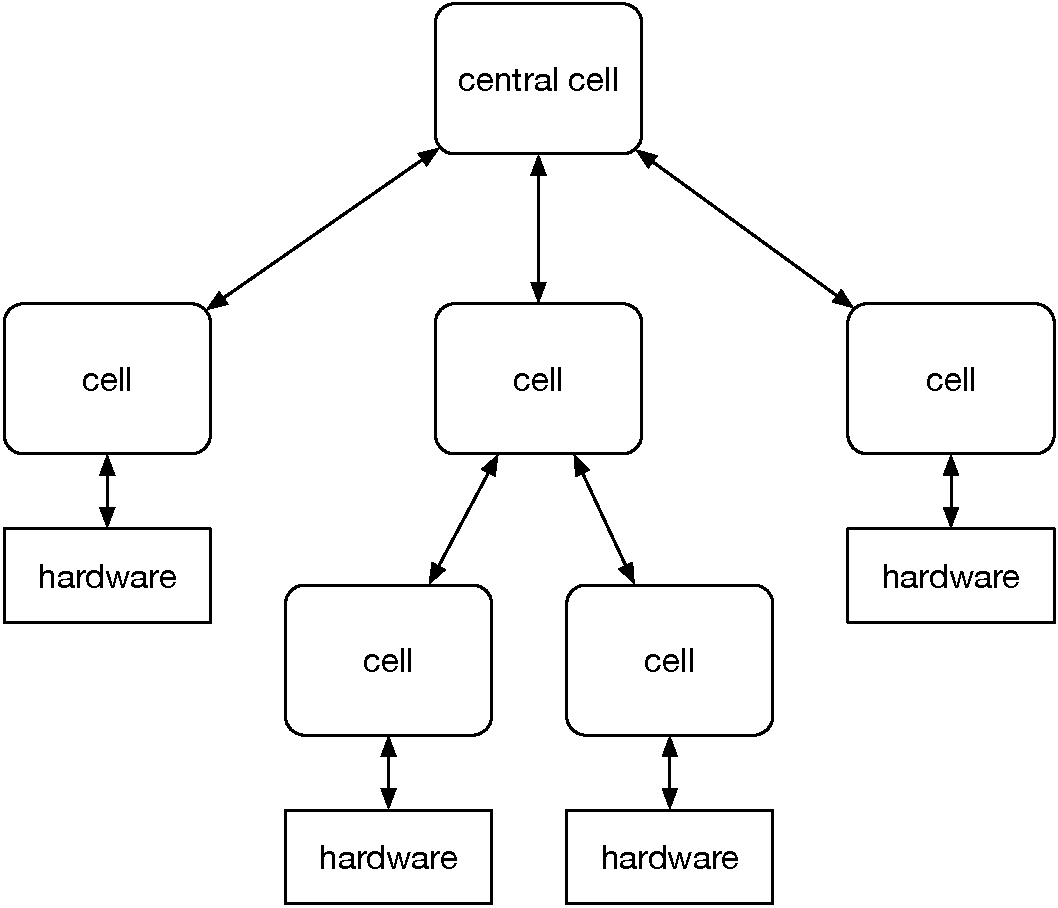
\includegraphics[width=.75\textwidth]{images/cell-tree}
  \caption{An example of the Trigger Supervisor Cell structure}
  \label{fig:cell-tree}
\end{figure}

\section{SWATCH}
The phase II upgrades of LHC will increase the luminosity of the produced beams.
This means there will be more proton-proton collisions per bunch crossing in the
experiment, which in turn means there is a bigger amount of data that needs
processing.

To support this increase of collision rates, the current hardware at CMS needs
to be adapted or replaced to support the higher data rate.

The SWATCH project (SoftWare for Automating conTrol Common Hardware) is an
endeavor to standardize the communication with boards and the functions they
provide.
It attempts to exploit commonalities between hardware components and uses it
to provide a common high level API to greatly simplify the development of the
online software\cite{SWATCH}.
